\begin{filecontents}[overwrite,noheader]{references.bib}
@article{robinson2019digital,
  title={Digital fundraising: How technology is transforming charitable giving},
  author={Robinson, David},
  journal={Journal of Nonprofit and Public Sector Marketing},
  volume={31},
  number={4},
  pages={377--392},
  year={2019},
  publisher={Taylor and Francis}
}

@article{sandhu1996rbac,
  title={Role-based access control models},
  author={Sandhu, Ravi S and Coyne, Edward J and Feinstein, Hal L and Youman, Charles E},
  journal={IEEE Computer},
  volume={29},
  number={2},
  pages={38--47},
  year={1996},
  publisher={IEEE}
}

@article{sander2021digital,
  title={The Digital Transformation of Fundraising: Key Technology Trends and Implications for Nonprofit Organizations},
  author={Sander, Jutta},
  journal={Nonprofit Management and Leadership},
  volume={32},
  number={1},
  pages={15--35},
  year={2021},
  publisher={Wiley Periodicals, Inc.}
}

@inproceedings{huang2020online,
  title={An Online Donation System Based on Blockchain and Smart Contract},
  author={Huang, Jianping and Lu, Yujia and Chen, Kai and Zheng, Min and Liu, Jinlong},
  booktitle={2020 IEEE International Conference on Services Computing (SCC)},
  pages={102--109},
  year={2020},
  organization={IEEE}
}

@article{barnes2018rise,
  title={The Rise of Crowdfunding and Digital Fundraising: A Nonprofit's Guide to Success},
  author={Barnes, Christopher},
  journal={Journal of Nonprofit and Public Sector Marketing},
  volume={30},
  number={4},
  pages={430--445},
  year={2018},
  publisher={Taylor and Francis}
}

@book{schlegelmilch2022strategic,
  title={Strategic International Fundraising},
  author={Schlegelmilch, Bodo B and Penz, Elfriede and Kizilgun, Meltem},
  year={2022},
  publisher={Routledge},
  note={Focuses on the role of digital platforms in global giving.}
}

@article{sanchez2019framework,
  title={A Conceptual Framework for Implementing Secure and Transparent E-Donation Systems},
  author={Sanchez, Juan and Gutierrez, Ricardo and Martinez, Isabel},
  journal={International Journal of Computer Science and Information Security},
  volume={17},
  number={7},
  pages={112--120},
  year={2019}
}

@inproceedings{wang2021enhancing,
  title={Enhancing Donor Engagement and Retention through Personalized Digital Experience},
  author={Wang, Lin and Zhang, Wei},
  booktitle={Proceedings of the International Conference on E-business and E-commerce (ICEC)},
  pages={55--62},
  year={2021},
  organization={ACM}
}

@article{smith2020tech,
  title={Tech-Enabled Volunteer Management: Optimizing Coordination and Reporting for Nonprofits},
  author={Smith, Abigail},
  journal={Volunteer Management Journal},
  volume={25},
  number={3},
  pages={78--90},
  year={2020}
}

@article{jones2023modern,
  title={Modern Web Development Stacks for Enterprise Applications: A Comparison of .NET, React, and Angular},
  author={Jones, Robert and Miller, Sarah},
  journal={Journal of Software Engineering and Applications},
  volume={16},
  number={4},
  pages={135--150},
  year={2023}
}

@article{chen2022machine,
  title={Machine Learning Applications in Nonprofit Fundraising: Predictive Analytics for Donor Behaviour},
  author={Chen, Wei and Liu, Xiaoming},
  journal={Journal of Nonprofit Technology and Innovation},
  volume={8},
  number={2},
  pages={45--67},
  year={2022}
}

@inproceedings{ahmed2021anomaly,
  title={Anomaly Detection in Financial Transactions Using Isolation Forest and Singular Spectrum Analysis},
  author={Ahmed, Salman and Khan, Bilal},
  booktitle={Proceedings of the International Conference on Financial Data Engineering},
  pages={88--96},
  year={2021},
  organization={IEEE}
}

@article{gupta2020donor,
  title={Predicting Donor Attrition in Charitable Organizations Using Supervised Machine Learning},
  author={Gupta, Priya and Sharma, Amit},
  journal={International Journal of Data Science and Analytics},
  volume={10},
  number={3},
  pages={211--225},
  year={2020}
}

@book{freeman2021react,
  title={Pro React 18 with TypeScript: Building Enterprise-Grade Applications},
  author={Freeman, Adam},
  year={2021},
  publisher={Apress},
  address={New York, NY}
}

@book{lock2021aspnet,
  title={ASP.NET Core in Action},
  author={Lock, Andrew},
  edition={2nd},
  year={2021},
  publisher={Manning Publications},
  address={Shelter Island, NY}
}

@book{lerman2020efcore,
  title={Programming Entity Framework Core: Data Access for .NET Applications},
  author={Lerman, Julie and Miller, Rowan},
  year={2020},
  publisher={O'Reilly Media},
  address={Sebastopol, CA}
}

@article{suoranta2019otp,
  title={OTP-Based Multi-Factor Authentication: Security Challenges and Implementation Strategies in Web Applications},
  author={Suoranta, Sanna and Toivonen, Antero},
  journal={Journal of Internet Security and Privacy},
  volume={7},
  number={1},
  pages={12--28},
  year={2019}
}

@inproceedings{provos1999bcrypt,
  title={A Future-Adaptable Password Scheme},
  author={Provos, Niels and Mazieres, David},
  booktitle={USENIX Annual Technical Conference Proceedings},
  pages={81--91},
  year={1999},
  organization={USENIX Association}
}

@article{rathore2021volunteer,
  title={Digital Platforms for Volunteer Management: Enhancing Engagement and Retention in Nonprofit Organizations},
  author={Rathore, Ajay Kumar and Ilavarasan, P. Vigneswara},
  journal={VOLUNTAS: International Journal of Voluntary and Nonprofit Organizations},
  volume={32},
  number={4},
  pages={891--906},
  year={2021},
  publisher={Springer}
}

@article{beck2001agile,
  title={Manifesto for Agile Software Development},
  author={Beck, Kent and Beedle, Mike and van Bennekum, Arie and Cockburn, Alistair and Fowler, Martin and others},
  journal={Agile Alliance},
  year={2001},
  note={Available at: https://agilemanifesto.org}
}

@article{kalinda2022university,
  title={University-Based Donation Platforms: Challenges and Opportunities for Digital Transformation in Higher Education Philanthropy},
  author={Kalinda, Emmanuel and Mwase, Wilfred},
  journal={Journal of Higher Education Development},
  volume={15},
  number={2},
  pages={88--104},
  year={2022}
}

@inproceedings{hutto2014vader,
  title={{VADER}: A Parsimonious Rule-Based Model for Sentiment Analysis of Social Media Text},
  author={Hutto, Clayton and Gilbert, Eric},
  booktitle={Proceedings of the International AAAI Conference on Web and Social Media},
  volume={8},
  number={1},
  pages={216--225},
  year={2014},
  organization={AAAI Press}
}

@article{owasp2021top10,
  title={OWASP Top Ten Web Application Security Risks},
  author={{OWASP Foundation}},
  journal={Open Web Application Security Project},
  year={2021},
  note={Available at: https://owasp.org/Top10}
}

@article{iso27001security,
  title={Information Security Management: ISO/IEC 27001 Standard and Its Application in Software Systems},
  author={Disterer, Georg},
  journal={Journal of Information Security},
  volume={4},
  number={2},
  pages={92--100},
  year={2013}
}

@misc{jones2015jwt,
  title={JSON Web Token (JWT)},
  author={Jones, Michael B and Bradley, John and Sakimura, Nat},
  howpublished={RFC 7519, Internet Engineering Task Force},
  year={2015},
  note={Available at: https://tools.ietf.org/html/rfc7519}
}
\end{filecontents}

\documentclass{thesis-library}
   
\usepackage{lipsum}
\usepackage{float}
\setcode{utf8}

% Abbreviations List
\newacronym{dms}{DMS}{Donation Management System}
\newacronym{cse}{CSE}{Computer Science and Engineering}

% Variable
\newcommand{\projectTitle}{\textbf{Donation Management System}}

\begin{document}
\newcommand{\thesisTitle}{Campus Based Donation Management System}

\newcommand{\byLabel}{\underline{Submitted By}}
\newcommand{\studentID}{Student ID: 200114}
\newcommand{\studentRegYear}{Registration Year: 2020-21}
\newcommand{\studentName}{Ramjan Ali Kha}
\newcommand{\supervisorLabel}{\underline{Supervisor}}
\newcommand{\supervisorName}{Dr. Mohammad Nowsin Amin Sheikh}
\newcommand{\supervisorDesig}{Assistant Professor}
\newcommand{\supervisorAff}{Department of Computer Science and Engineering}
\newcommand{\degreeLineALabel}{This project report was submitted in partial fulfillment of the}
\newcommand{\degreeLineBLabel}{Requirements for the BSc.Engg Degree}
\newcommand{\majorName}{In \textbf{Computer Science and Engineering.}}
\newcommand{\universityName}{Jashore University of Science and Technology}
\newcommand{\regionName}{Jashore-7408, Bangladesh}
\newcommand{\degreeyearName}{2025}
\newcommand{\degreemonthName}{November}
\newcommand{\approvalText}{This project titled \textbf{Campus Based} \textbf{Donation Management System}
submitted by \textbf{Ramjan Ali Kha} for progress defence for the degree of B.Sc. in Computer Science and
Engineering on November 23, 2025.}
\newcommand{\studentSign}{\underline{Signature of the Student}}
\newcommand{\supervisorSign}{\underline{Signature of the Supervisor}}

\makecoverpage
\makeapprovalpage

\pagenumbering{roman}

\chapter*{Acknowledgments}
\addcontentsline{toc}{chapter}{Acknowledgments}
I want to thank \textbf{Almighty Allah}, the Creator and the Sustained of the word, for providing us with the opportunity, capacity, energy, spirit, and patience to finish the report.
\\
I want to express my sincere gratitude to Dr. Mohammad Nowsin Amin Sheikh, assistant professor at Jashore University of Science and Technology and my respected educator and supervisor. His unwavering advice and direction were crucial to the success of this project. In order to make this project writing as perfect as possible, he was constantly offering valuable assistance. The completion of the report would not have been possible without his extensive knowledge, insightful ideas, boundless enthusiasm, invaluable advice, assistance, and suggestions. I am honored to have had the chance to work and study under his supervision.
\\
I also want to express my gratitude to the honorable faculty of the Department of Computer Science and Engineering. I appreciate their support and helpful criticism, which enabled me to write my project report more skillfully.
\\
My friends and family have been a major source of inspiration and passion for me, and for that I am incredibly grateful. All of their love, kindness, and support have been invaluable to me during this time.
\\
I would want to thank my parents and family for their unwavering support and motivation. I am grateful for your understanding, love, support, and patience, all of which inspired me to complete my studies.

\listofabbreviations

\tableofcontents

\newpage
\listoffigures
\newpage
\listoftables
\newpage
\chapter*{List of Acronyms}
\vspace{-40pt}
\begin{table}[h]
    \renewcommand{\arraystretch}{1.6}
    \centering
    \caption{\textbf{List of Acronyms.}}
    \vspace{10pt}
    \begin{tabular}{|l|l|}
        \hline
        \textbf{Acronyms} & \textbf{Full Form} \\
        \hline
        DMS & Donation Management System\\
        UI & User Interface\\
        API & Application Programming Interface\\
        CRUD & Create, Read, Update, Delete\\
        JWT & JSON Web Token\\
        ORM & Object-Relational Mapping\\
        REST & Representational State Transfer\\
        HTTPS & Hypertext Transfer Protocol Secure\\
        SQL & Structured Query Language\\
        EF & Entity Framework\\
        RBAC & Role Based Access Control\\
        HTML & Hypertext Markup Language\\
        CSS & Cascading Style Sheets\\
        TypeScript & Programming Language\\
        React & JavaScript Library\\
        Redux & State Management\\
        .NET & Framework\\
        C\# & Programming Language\\
        \hline
    \end{tabular}
\end{table}

\chapter*{Abstract}
\addcontentsline{toc}{chapter}{Abstract}
Non-governmental organizations and charitable institutions must execute their operational and financial activities efficiently to achieve their objectives. These methods encompass campaign coordination, transparent fundraising and resource distribution, and efficient volunteer administration. Nonetheless, numerous companies continue to depend on paper-based procedures and manual recordkeeping. While participating in fundraising initiatives for the 2024 Sylhet flood and the medical bills of our late sister Atika (CSE 17-18), I noted that these campaigns frequently result in inaccuracies, insufficient transparency, and superfluous bureaucratic complexities. The proposed Donation Management System (DMS) consolidates all pertinent functions into a unified, user-friendly software platform to tackle these difficulties.
\\
The system employs a novel, multi-layered architecture. ASP.NET Core Web API is utilized to establish a safe and resilient infrastructure, whereas React and TypeScript are employed to create a responsive and user-centric frontend. The solution employs Entity Framework Core alongside a relational database to provide effective data management and scalability.
\\
Security is essential and includes technologies such as BCrypt password hashing, CSRF protection, input validation, and secure payment processing. The responsive design guarantees interoperability across all devices, encompassing personal computers and mobile phones. The Donation Management System markedly decreases manual labor, improves transparency, and streamlines the implementation of donation campaigns for diverse organizations.
\\
The project includes features such as campaign management, donation processing, volunteer coordination, user authentication and access restriction, feedback sentiment analysis, and a physical donation tracking system. This technology aims to increase donor confidence and participation by promoting transparency and automating routine tasks to simplify the donation process. 

 
\\

\newpage
\pagenumbering{arabic}

\printchaptertitle{Introduction}
\newpage
\section{Overview} The \textbf{Campus Based Donation Management System} represents a multifaceted, web-centric architecture engineered to digitize and automate the operational paradigms associated with institutional philanthropy. Through the strategic integration of administrators, donors, and volunteers within a consolidated digital ecosystem, the framework mitigates the logistical frictions inherent in manual coordination by deploying a role-adaptive interface.
\\The platform encompasses a robust functional suite, categorized as follows: \begin{itemize} \item \textbf{Financial Administration:} Provisions for real-time transactional monitoring, seamless online payment integration via SSLCommerz, and secure physical donation authentication utilizing One-Time Password (OTP) protocols. \item \textbf{Operational Orchestration:} Systematic management of campaign lifecycles, meritocratic rank progression frameworks for volunteers, and the automation of expenditure voucher authorization workflows. \item \textbf{Predictive Intelligence:} The incorporation of a machine learning subsystem dedicated to forecasting longitudinal donation trends, identifying transactional anomalies, and modeling donor attrition probabilities. \end{itemize}
\\The platform's infrastructure is founded upon a contemporary multi-tier architectural design. The presentation layer leverages \textbf{React in conjunction with TypeScript} to ensure a responsive and type-safe user interface, while the application layer is sustained by an \textbf{ASP.NET Core Web API}. Data persistence and integrity are maintained through \textbf{Microsoft SQL Server} and Entity Framework Core. System security is rigorously enforced via JSON Web Token (JWT) authentication, BCrypt cryptographic hashing, and Role-Based Access Control (RBAC), establishing a scalable and resilient foundation designed for future iterative expansion.

\section{Background}
Charitable organizations and donation management initiatives have always relied on manual, paper-based systems or fragmented digital solutions to monitor donations, oversee campaigns, and coordinate volunteers. These traditional methods are frequently laborious, prone to errors, and ineffective. Common difficulties intrinsic to these systems include:

\begin{itemize} \item \textbf{Tracking Latency:} Significant institutional impediments regarding the real-time surveillance of philanthropic contributions and the temporal tracking of campaign progression. \end{itemize}

\begin{itemize} \item \textbf{Data Redundancy:} Systemic data redundancies and clerical inconsistencies derived from a reliance on non-automated, manual data procurement protocols. \end{itemize}

\begin{itemize} \item \textbf{Operational Inefficiency:} Suboptimal operational coordination and the absence of empirical metrics for monitoring individual volunteer engagement and resource contributions. \end{itemize}

\begin{itemize} \item \textbf{Analytical Deficiencies:} Methodological constraints in the quantitative assessment of donor behavioral patterns and the empirical evaluation of campaign efficacy. \end{itemize}

\begin{itemize} \item \textbf{Obstacles to Communication:} A deficiency in established, bidirectional communication channels between philanthropic organizations and their respective donor cohorts. \end{itemize}

\begin{itemize} \item \textbf{Lack of Transparency:} Informational opacity concerning fund utilization, which correlates with diminished stakeholder trust and attenuated longitudinal institutional engagement. \end{itemize}

\begin{itemize} \item \textbf{No Financial Accountability:} A pervasive lack of robust audit trails and standardized financial reporting frameworks, complicating the verification of fund-disbursement alignment with organizational objectives. \end{itemize}

\begin{itemize} \item \textbf{Limited Donor Visibility:} Restricted donor access to real-time metrics regarding campaign trajectory, financial utilization, and social impact, thereby disincentivizing recurring philanthropic participation. \end{itemize}

\begin{itemize} \item \textbf{Absence of Physical Donation Management:} The absence of formalized protocols for the systematic documentation, verification, and longitudinal tracking of in-kind assets, leading to unrecorded philanthropic capital and compromised institutional accountability. \end{itemize}

\begin{itemize} \item \textbf{Inadequate Expense Voucher Oversight:} Deficiencies in structured expenditure oversight and formalized voucher authorization workflows, which impede the monitoring and validation of campaign-related operational costs. \end{itemize}

\begin{itemize} \item \textbf{Unregulated Fund Withdrawal Processes:} Non-regulated fiscal disbursement protocols and a lack of controlled reserve fund management, increasing institutional vulnerability to fund misappropriation and undermining the integrity of financial audit trails. \end{itemize}

\begin{itemize} \item \textbf{Absence of Predictive and Analytical Capabilities:} A prevailing reliance on reactive data architectures that lack the predictive intelligence necessary for forecasting donation trends, detecting transactional anomalies, or modeling donor attrition—capabilities essential for evidence-based strategic planning. \end{itemize}

\begin{itemize} \item \textbf{Lack of Volunteer Recognition and Incentivization:} The deficiency of formalized meritocratic progression and achievement recognition frameworks, which adversely impacts volunteer motivation and longitudinal retention within mission-driven philanthropic initiatives. \end{itemize}

\begin{itemize} \item \textbf{Insufficient Automated Notification Infrastructure:} Inadequate automated notification infrastructures that result in unreliable communication workflows, failing to provide the instantaneous updates such as contribution confirmations and secure authentication protocols requisite for maintaining institutional credibility. \end{itemize} \\ Driven by the rapid proliferation of digital transformation and the intensification of stakeholder requirements for sophisticated online interfaces, organizations recognize the imperative for centralized, automated architectures. The proposed Donation Management System addresses these systemic lacunae by providing a comprehensive digital framework that streamlines critical operations while upholding rigorous standards of data confidentiality, financial transparency, and user inclusivity. 

\section{Motivation}
The impetus for the development of the Donation Management System originates from the pervasive operational inefficiencies inherent in traditional philanthropic administrative workflows. Contemporary charitable organizations frequently encounter significant structural challenges in several critical domains: \begin{itemize} \item The concurrent orchestration of heterogeneous donation streams and diverse payment modalities. \item The systematic monitoring of volunteer engagement and the empirical quantification of their respective social impacts. \item The diagnostic evaluation of campaign efficacy and the qualitative assessment of donor sentiment through structured feedback mechanisms. \item The dissemination of instantaneous, longitudinal updates to stakeholders regarding the trajectory of specific philanthropic initiatives. \item The maintenance of high-integrity, secure repositories for fiscal transactional records and sensitive donor data. \end{itemize}
\\This initiative seeks to architect a sophisticated, scalable framework that mitigates these systemic bottlenecks while establishing a robust foundation for future iterative innovations in philanthropic management. By leveraging cutting-edge web technologies and adhering to rigorous software architectural standards, the system ensures high operational reliability, robust security protocols, and optimal user satisfaction.

\section{Problem Statement}

Organizations tasked with the administration of philanthropic initiatives encounter multifaceted operational impediments arising from manual and fragmented data architectures: \begin{itemize} \item \textbf{Absence of Real-Time Surveillance:} Significant temporal information gaps prevent both donors and administrative entities from monitoring campaign trajectories and contribution statuses in real-time. \item \textbf{Manual Fiscal Procurement:} Non-automated donation collection modalities are inherently inefficient, susceptible to clerical error, and present substantial security vulnerabilities. \item \textbf{Fragmentation in Human Capital Orchestration:} The lack of a centralized management framework complicates the coordination of volunteer cohorts, the tracking of individual engagement, and the empirical quantification of their respective social impacts. \item \textbf{Systemic Data Integrity Vulnerabilities:} Manual record-keeping protocols lead to pervasive data inconsistencies, undermining the generation of accurate, high-fidelity reports for institutional oversight. \item \textbf{Methodological Constraints in Analytics:} Administrative bodies lack the diagnostic tools necessary to generate insights into donor behavioral patterns, campaign efficacy, and the sentiment analysis of stakeholder testimonials. \item \textbf{Security and Cryptographic Risks:} Conventional systems and unencrypted digital repositories pose significant risks to the confidentiality and integrity of sensitive financial records and donor profiles. \item \textbf{Institutional Opacity:} Contemporary frameworks frequently lack transparency mechanisms; donor motivation is empirically linked to the visibility of tangible outcomes and the precise verification of fund expenditures. \item \textbf{Deficiency in Integrated Fiscal Accounting:} Existing localized systems typically lack integrated bookkeeping modules, preventing the synchronization of donation inflows with formal ledger management. \end{itemize}
\\The implementation of an automated, web-centric management architecture is an imperative requirement to mitigate these systemic lacunae, providing a resilient, transparent, and efficacious environment for the administration of philanthropic capital and mission-driven campaigns.

\section{Questions Addressed by the Project}

The project seeks to address the following research questions:
\begin{itemize}
    \item How can a unified web-based system improve donation collection, tracking, and campaign management?
    \item What are the benefits of implementing role-based access control for multiple user types in a donation management context?
    \item How effective is real-time donation tracking in improving campaign transparency and donor satisfaction?
    \item To what extent does an integrated and secure online payment module streamline the donation process?
    \item How can sentiment analysis on donor testimonials provide insights into campaign impact and donor satisfaction?
    \item What database management and security techniques are most effective in protecting sensitive donor information?
\end{itemize}

\newpage
\section{Objectives}
The following are the main objectives of the Donation Management System:
\begin{itemize}
    \item \textbf{To provide a unified web-based platform} that streamlines donation collection, campaign management, volunteer coordination, and reporting.
    \item \textbf{To implement role-based access control} with distinct functions for Admins, Donors, Volunteers, and Campaign Creators.
    \item \textbf{To offer real-time donation and campaign tracking} that provides transparency and immediate feedback to stakeholders.
    \item \textbf{To integrate secure payment processing} using SSLCommerz gateway for safe and efficient transaction handling.
    \item \textbf{To improve user experience} with a responsive, intuitive interface accessible across all devices.
    \item \textbf{To ensure data security and integrity} through proper authentication, encryption, and validation mechanisms.
    \item \textbf{To enable sentiment analysis} on donor testimonials to measure campaign impact and donor satisfaction.
    \item \textbf{To provide comprehensive reporting and analytics} for decision-making and performance tracking.
\end{itemize}

\newpage
\section{Organization}

The Donation Management System development process is presented methodically in each of the six chapters that make up this project report. The report's structure is as follows:

\textbf{Chapter 1: Introduction} - Overview, background, motivation, problem statement, objectives, and organization.

\textbf{Chapter 2: Background and Related Technologies} - Existing systems, relevant technologies, and identified gaps.

\textbf{Chapter 3: Methodology} - System design, development process, testing, deployment, and security measures.

\textbf{Chapter 4: System Architecture and Design} - Frontend, backend, database design, and system diagrams (ER, Use Case, Schema).

\textbf{Chapter 5: Implementation} - System setup, technologies used, and implementation of key modules.

\textbf{Chapter 6: Conclusion and Future Work} - Summary and recommendations for future enhancements.


\printchaptertitle{Background and Related Technologies}
\section{Overview} In the context of the escalating global dynamics of digital transformation, organizations are progressively transitioning towards automated frameworks to improve administrative governance and the effectiveness of service delivery. Philanthropic management paradigms have experienced a longitudinal evolution from traditional manual documentation practices to advanced digital ecosystems meticulously designed to enhance operational efficacy and stakeholder involvement \cite{sander2021digital}. This chapter conducts a thorough analysis of current donation management practices and emergent technological frameworks, ultimately recognizing the systemic deficiencies that the proposed Donation Management System (DMS) aims to address.

\section{Traditional Donation Management Methods}

Conventional donation management typically relies on manual processes including paper-based records, in-person collection, and spreadsheet tracking. These methods present significant challenges \cite{robinson2019digital}:
\begin{itemize}
    \item Difficulty in real-time donation tracking and campaign monitoring.
    \item Increased likelihood of errors and data loss.
    \item Inefficient resource allocation for volunteer coordination.
    \item Limited ability to analyze campaign effectiveness.
    \item Security risks associated with physical records and unencrypted digital storage.
\end{itemize}

\section{Existing Digital Donation Management Solutions}

Several commercial donation management platforms exist, including:
\\
\textbf{Donorbox:} Cloud-based donation platform with payment processing and donor management \cite{barnes2018rise}.
\\
\textbf{GiveWP:} WordPress-integrated donation plugin with customizable forms.
\\
\textbf{Network for Good:} Comprehensive fundraising and donor management platform \cite{schlegelmilch2022strategic}.
\\
These solutions, while effective for many organizations, often lack customization for specific institutional needs, are costly, and may not integrate seamlessly with existing systems used by smaller organizations \cite{sanchez2019framework}. Advanced solutions also explore secure and transparent e-donation systems using technologies like Blockchain \cite{huang2020online}.

\section{Role-Based Access Control in Management Systems}

Role-Based Access Control (RBAC) is essential for multi-user platforms \cite{sandhu1996rbac}. RBAC provides:
\begin{itemize}
    \item \textbf{Security:} Restricts access to sensitive information based on user roles.
    \item \textbf{Usability:} Displays only features relevant to each user's responsibilities.
    \item \textbf{System Integrity:} Prevents unauthorized modifications.
\end{itemize}
\\The Donation Management System implements RBAC for Admins (full system access), Donors (donation and profile management), Volunteers (activity reporting), and Campaign Creators (campaign management).

\section{Payment Gateway Integration}

Secure online payment processing is critical for donation platforms. SSLCommerz, a popular payment gateway in South Asia, provides:
\begin{itemize}
    \item Multiple payment method support (credit card, mobile banking, wallet).
    \item Secure transaction processing and encryption.
    \item Real-time payment confirmation and callback notifications.
    \item Comprehensive transaction reporting.
\end{itemize}

\section{Sentiment Analysis in Donation Systems}

Sentiment analysis provides organizations with insights into donor satisfaction and campaign impact \cite{hutto2014vader}. Using TextBlob or similar natural language processing libraries, testimonials can be automatically classified as positive, negative, or neutral \cite{wang2021enhancing}, enabling:
\begin{itemize}
    \item Measurement of campaign effectiveness through donor feedback.
    \item Identification of areas for improvement.
    \item Data-driven decision-making for future campaigns.
\end{itemize}

\section{Modern Web Technologies}

The Donation Management System leverages contemporary web development technologies \cite{jones2023modern}:
\begin{itemize}
    \item \textbf{Frontend:} React with TypeScript \cite{freeman2021react}, Redux Toolkit for state management, Tailwind CSS for styling.
    \item \textbf{Backend:} ASP.NET Core Web API for building scalable RESTful services \cite{lock2021aspnet}.
    \item \textbf{Database:} SQL Server for robust relational data management and Entity Framework Core for ORM \cite{lerman2020efcore}.
    \item \textbf{Authentication:} JWT tokens for stateless authentication and OTP-based email and SMS verification \cite{suoranta2019otp}.
    \item \textbf{Security:} BCrypt for password hashing \cite{provos1999bcrypt}, CSRF tokens for form protection, input validation and sanitization \cite{owasp2021top10}.
\end{itemize}
These technologies are critical for ensuring system scalability and maintainability \cite{smith2020tech}.

\section{Identified Gaps}

While existing solutions provide valuable features, gaps remain in:
\begin{itemize}
    \item Customization for organization-specific workflows and requirements, particularly in campus and higher-education contexts \cite{kalinda2022university}.
    \item Integration of machine learning capabilities such as donor attrition prediction and donation forecasting \cite{chen2022machine, gupta2020donor}.
    \item Anomaly detection in financial transactions to safeguard campaign integrity \cite{ahmed2021anomaly}.
    \item Structured volunteer recognition frameworks to improve long-term retention \cite{rathore2021volunteer}.
    \item Cost-effectiveness for smaller organizations and educational institutions.
    \item Flexibility in feature selection and deployment options.
\end{itemize}

The Donation Management System addresses these gaps by providing a customizable, feature-rich platform tailored to diverse organizational needs.

\printchaptertitle{Methodology}
\section{Overview}
This chapter describes the design, development, testing, and implementation of the Donation Management System. It outlines the technological stack, system architecture, and development methodologies employed.

\section{System Design}
 Developing a solid, scalable, and intuitive architecture that supports various user roles while
 preserving security and performance is the major goal of the system design process. The front
 end, back-end, and database design are the three primary components of the design phase.

\subsection{Frontend Design}
The frontend is built using React with TypeScript, ensuring type safety and code maintainability. Key design principles include:
\begin{itemize}
    \item \textbf{Responsive Design:} Utilizes CSS Flexbox and media queries for cross-device compatibility.
    \item \textbf{Component-Based Architecture:} Reusable React components for efficient development.
    \item \textbf{State Management:} Redux Toolkit for predictable and efficient state management.
    \item \textbf{Accessibility:} Follows WCAG guidelines for inclusive design.
\end{itemize}

\subsection{Backend Design}
The backend utilizes .NET Core Web API with an MVC architecture:
\begin{itemize}
    \item \textbf{Controllers:} Handle HTTP requests and business logic.
    \item \textbf{Models:} Define data structures and relationships.
    \item \textbf{Services:} Encapsulate business logic and operations.
    \item \textbf{Middleware:} Implement authentication, authorization, and error handling.
\end{itemize}

\subsection{Database Design}
SQL Server with Entity Framework Core provides:
\begin{itemize}
    \item Relational data modeling with enforced referential integrity.
    \item Seven main entities: Users, Campaigns, Donations, Testimonials, Volunteers, VolunteerReports, CampaignUpdates.
    \item Indexed queries for performance optimization.
\end{itemize}

\section{Development Process}

The project follows Agile methodology with iterative development sprints, allowing continuous feedback incorporation and incremental feature delivery \cite{beck2001agile}.

\subsection{Frontend Development}
Role-specific interfaces were developed for:
\begin{itemize}
    \item \textbf{Admin:} Dashboard, user management, analytics, campaign management.
    \item \textbf{Donor:} Donation interface, testimonial submission, profile management.
    \item \textbf{Volunteer:} Activity reporting, campaign tracking, hour submission.
    
\end{itemize}

\subsection{Backend Development}
Key modules include:
\begin{itemize}
    \item \textbf{Authentication:} JWT-based authentication with role-based authorization.
    \item \textbf{Donation Processing:} Donation creation, SSLCommerz payment integration, transaction tracking.
    \item \textbf{Campaign Management:} CRUD operations, progress tracking, volunteer coordination.
    \item \textbf{Sentiment Analysis:} Testimonial processing with TextBlob for sentiment classification.
    \item \textbf{Analytics:} Aggregation of donation data, campaign metrics, volunteer statistics.
\end{itemize}

\section{Testing}

Comprehensive testing includes:
\begin{itemize}
    \item \textbf{Unit Testing:} Individual component and function testing.
    \item \textbf{Integration Testing:} Module interaction and API endpoint testing.
    \item \textbf{Security Testing:} Authentication, authorization, and data protection validation.
    \item \textbf{Performance Testing:} Load testing and response time optimization.
\end{itemize}

\section{Deployment}

Deployment considerations include:
\begin{itemize}
    \item Frontend deployment to CDN or static hosting.
    \item Backend deployment to cloud services (Azure, AWS).
    \item Database configuration and migration management.
    \item SSL certificate installation for HTTPS security.
    \item Environment configuration and secrets management.
\end{itemize}

\section{Security Measures}

Security is implemented throughout the system in accordance with established security standards \cite{iso27001security, owasp2021top10}:
\begin{itemize}
    \item \textbf{Authentication:} JWT tokens with secure token refresh mechanisms.
    \item \textbf{Password Security:} BCrypt hashing with salt \cite{provos1999bcrypt}.
    \item \textbf{CSRF Protection:} Token-based CSRF prevention.
    \item \textbf{Input Validation:} Server-side and client-side validation.
    \item \textbf{Data Encryption:} HTTPS for data transmission, encrypted storage for sensitive data.
    \item \textbf{Access Control:} Role-based authorization middleware.
\end{itemize}

\printchaptertitle{System Architecture and Design}
\section{Overview}
This chapter describes the Donation Management System's architecture, encompassing frontend design, backend architecture, database structure, and system diagrams that illustrate system components and their interactions.

\section{Frontend Architecture}
The frontend employs a component-based architecture with Redux for state management:
\begin{itemize}
    \item React components for UI rendering.
    \item Redux store for centralized state management.
    \item Tailwind CSS for styling and responsiveness.
    \item TypeScript for type safety and code quality.
\end{itemize}

\section{Backend Architecture}
The .NET Core Web API follows RESTful principles with clear separation of concerns:
\begin{itemize}
    \item Controllers handle HTTP requests and responses.
    \item Services implement business logic and operations.
    \item Repositories abstract data access operations.
    \item Middleware handles cross-cutting concerns.
\end{itemize}

\section{Database Schema}
The system uses seven primary entities:
\begin{itemize}
    \item \textbf{Users:} User accounts with role assignments and authentication data.
    \item \textbf{Campaigns:} Fundraising campaigns with targets and progress tracking.
    \item \textbf{Donations:} Individual donation records linked to campaigns and donors.
    \item \textbf{Testimonials:} Donor testimonials with ratings and sentiment scores.
    \item \textbf{Volunteers:} Volunteer profiles and skill information.
    \item \textbf{VolunteerReports:} Activity logs and hour submissions.
    \item \textbf{CampaignUpdates:} Progress updates and campaign communications.
\end{itemize}

\section{ER Diagram}
The Entity-Relationship diagram illustrates the relationships between system entities and their attributes, showing one-to-many and one-to-one relationships between tables.

\begin{figure}[H]
  \centering
  \fbox{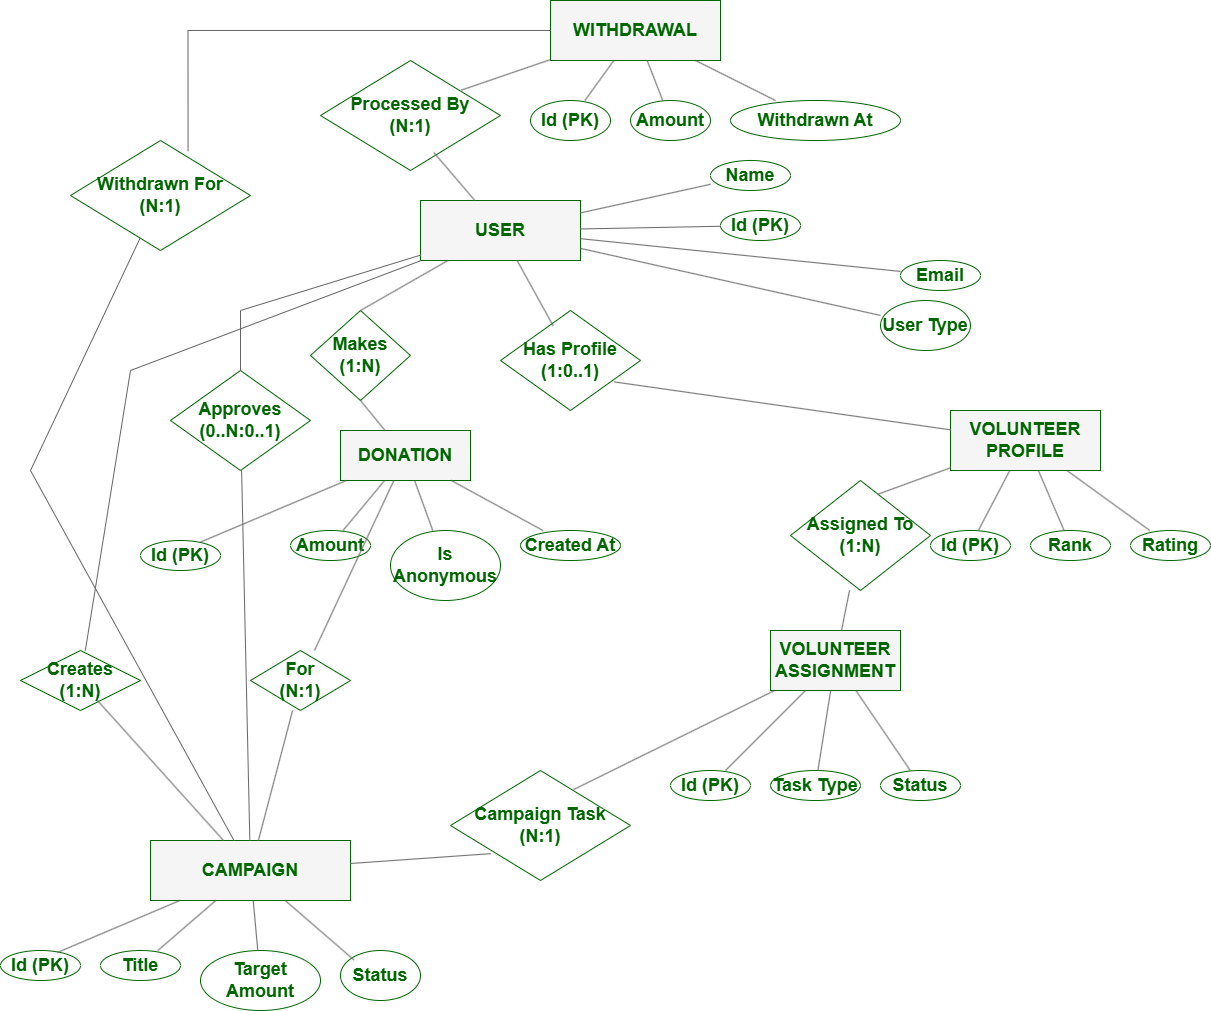
\includegraphics[width=1\textwidth]{images/er_diagram.png}}
  \caption{\textbf{Entity-Relationship Diagram.}}
\end{figure}

\section{Use Case Diagram}
The Use Case diagram depicts interactions between user roles (Admin, Donor, Volunteer, Campaign Creator) and system functionalities:

\begin{figure}[H]
  \centering
  \fbox{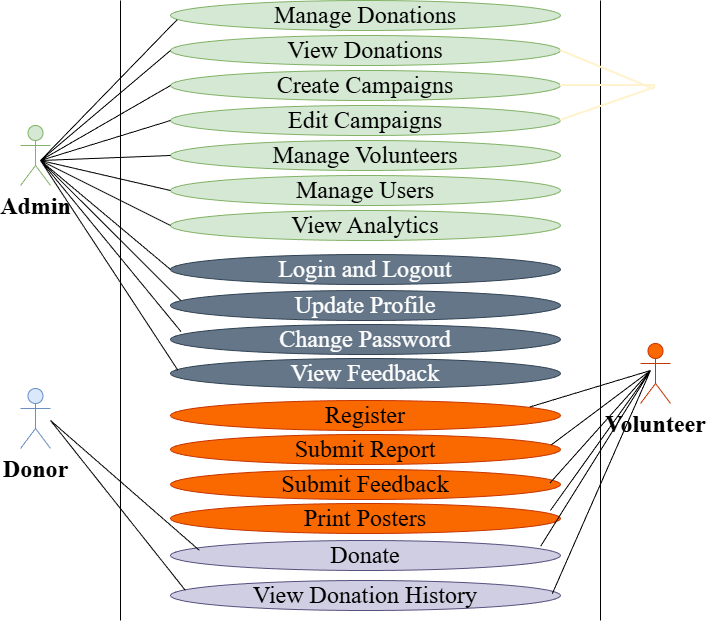
\includegraphics[width=1\textwidth]{images/use_case_diagram.png}}
  \caption{\textbf{Use Case Diagram.}}
\end{figure}

\section{Schema Diagram}
The Database Schema diagram shows the detailed structure of all tables, including fields, data types, and relationships:

\begin{figure}[H]
  \centering
  \fbox{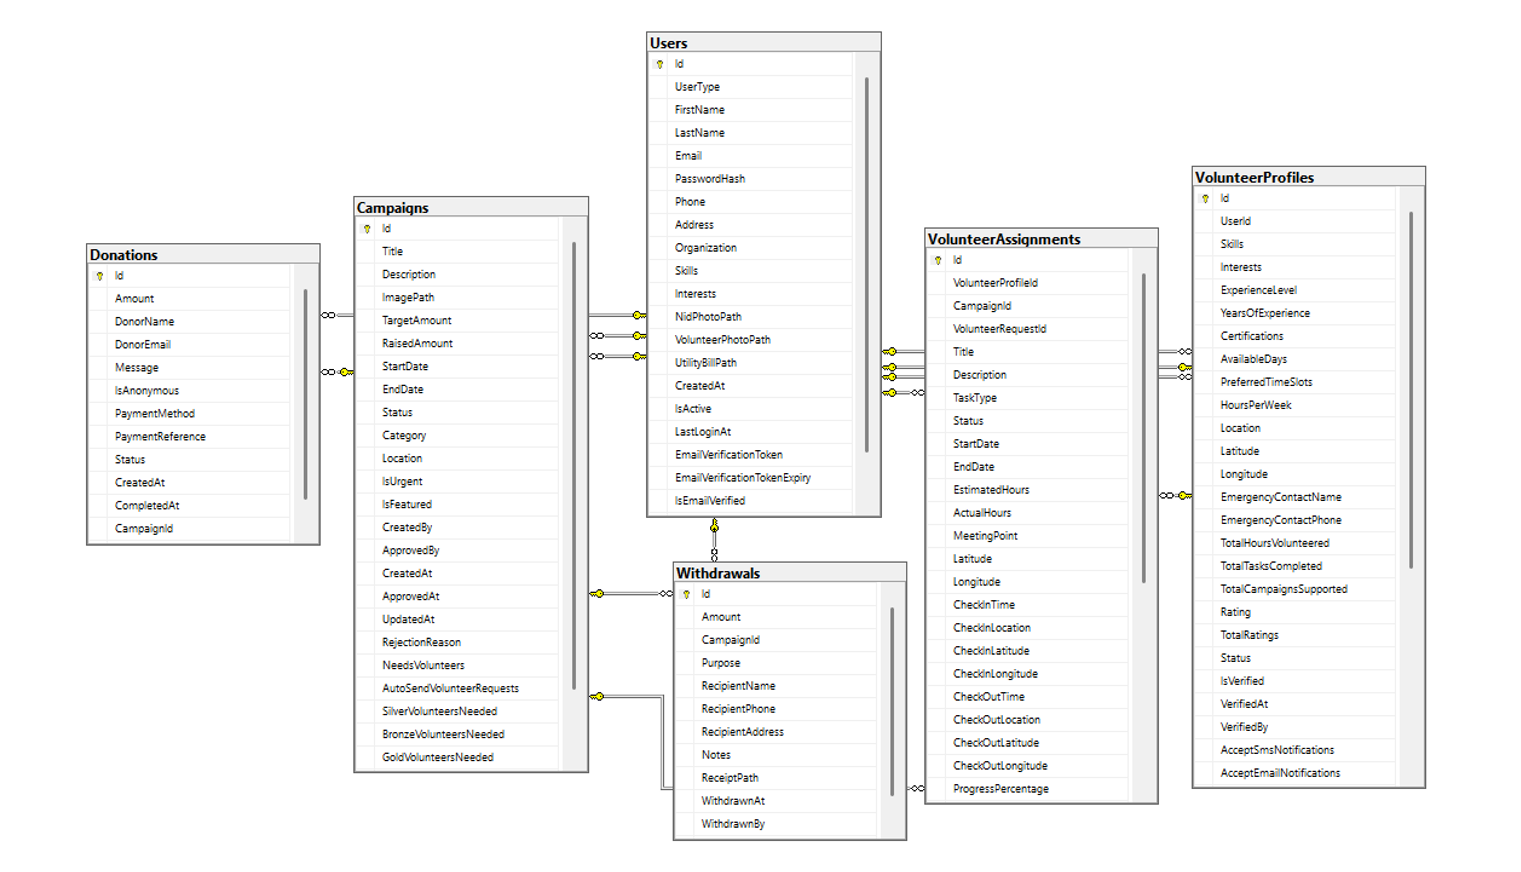
\includegraphics[width=1\textwidth]{images/schema_diagram.png}}
  \caption{\textbf{Database Schema Diagram.}}
\end{figure}

\section{Authentication Flow}
The system implements JWT-based authentication \cite{jones2015jwt}:
\begin{itemize}
    \item User credentials verified against hashed passwords.
    \item JWT token issued upon successful authentication.
    \item Token included in subsequent requests for authorization.
    \item Role-based middleware validates user permissions.
\end{itemize}

\section{Payment Processing Flow}
Integration with SSLCommerz gateway:
\begin{itemize}
    \item Donation request initiated by user.
    \item Redirect to SSLCommerz payment gateway.
    \item Payment processed securely.
    \item Callback notification received and verified.
    \item Donation record created upon successful payment.
\end{itemize}

\printchaptertitle{System Implementation}

\section{System Setup}
The implementation of the Donation Management System involves deploying a comprehensive web application with distinct frontend and backend components.

\subsection{Technologies Used}

\textbf{Frontend Technologies:}
\vspace{5pt}
\begin{table}[H]
    \centering
    \caption{\textbf{Frontend Technologies.}}
    \vspace{10pt}
    \begin{tabular}{|c|c|}
        \hline
        \textbf{SN} & \textbf{Technology} \\
        \hline
        1  & React \\
        2  & TypeScript \\
        3  & Redux Toolkit \\
        4  & Tailwind CSS \\
        5  & Axios (HTTP Client) \\
        6  & Vite (Build Tool) \\
        \hline
    \end{tabular}
\end{table}
\vspace{10}

\textbf{Backend Technologies:}
\vspace{5pt}
\begin{table}[H]
    \centering
    \caption{\textbf{Backend Technologies.}}
    \vspace{10pt}
    \begin{tabular}{|c|c|}
        \hline
        \textbf{SN} & \textbf{Technology} \\
        \hline
        1  & .NET Core 7/8 \\
        2  & C\# \\
        3  & Entity Framework Core \\
        4  & SQL Server \\
        5  & ASP.NET Core Identity \\
        6  & JWT Authentication \\
        \hline
    \end{tabular}
\end{table}
\vspace{10}

\section{System Implementation}

\subsection{Dashboard Overview}
The Admin Dashboard provides a comprehensive overview of system metrics, campaign status, donation progress, and volunteer activity. It displays real-time statistics for informed decision-making.

\begin{figure}[H]
  \centering
  \fbox{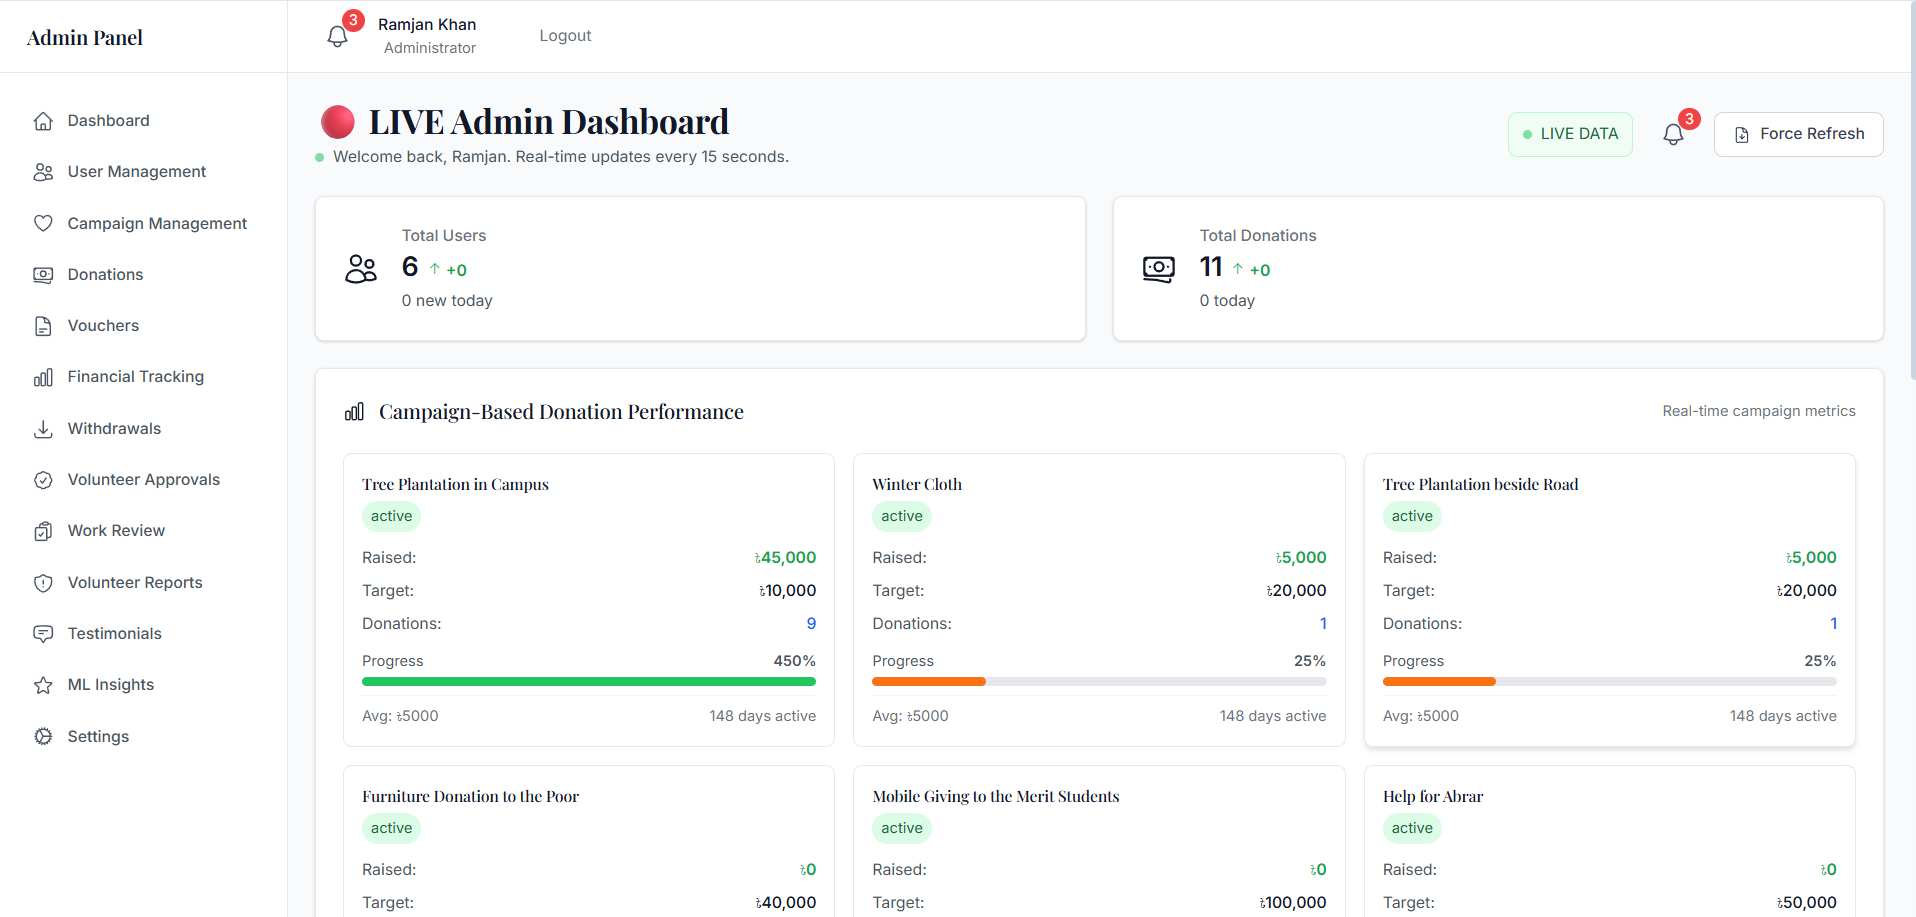
\includegraphics[width=1\textwidth]{images/admin_dashboard.png}}
  \caption{\textbf{Admin Dashboard.}}
\end{figure}

\subsection{Campaign Management}
Campaign creators can establish new campaigns, set fundraising targets, upload promotional materials, track progress, and post updates. The system monitors campaign status and provides real-time fundraising metrics.

\subsection{Donation Processing}
The donation module integrates SSLCommerz payment gateway, supporting multiple payment methods. Donors can make contributions securely, receive confirmations, and track their donation history through their profile.

\subsection{Volunteer Management}
Volunteers can register, submit activity reports with hour tracking, and monitor their contributions. Admins can approve submissions, track volunteer impact, and generate volunteer activity reports.

\subsection{Testimonial and Sentiment Analysis}
The system collects donor testimonials with ratings and feedback. Sentiment analysis automatically classifies testimonials, providing organizations with insights into donor satisfaction and campaign effectiveness.

\subsection{User Authentication}
Secure user authentication implements JWT tokens with email verification. Users authenticate with credentials, receive JWT tokens, and maintain sessions securely with automatic token refresh.

\subsection{Analytics and Reporting}
The Analytics module provides comprehensive reports on donation trends, campaign performance, volunteer contributions, and donor demographics. Data visualization helps stakeholders understand system performance and impact.

\begin{figure}[H]
  \centering
  \fbox{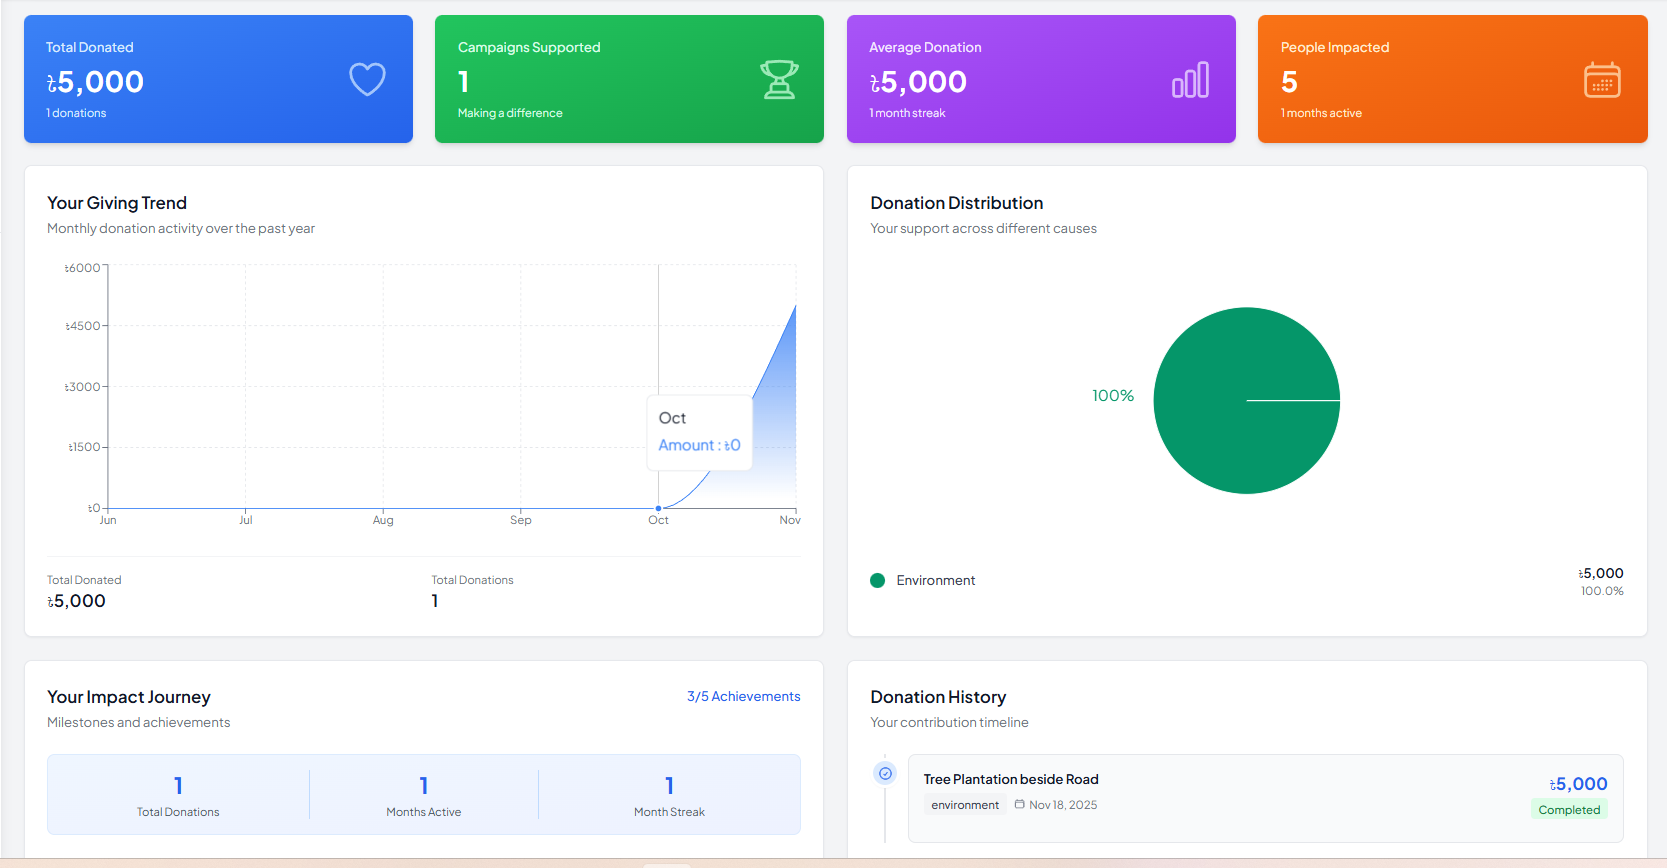
\includegraphics[width=1\textwidth]{images/analytics_dashboard.png}}
  \caption{\textbf{Analytics Dashboard.}}
\end{figure}

\section{Key Features Implementation}

\subsection{Donation Tracking}
Real-time donation tracking displays campaign progress toward targets, tracks individual donations, and provides transparency to donors and campaign creators.

\subsection{Campaign Updates}
Campaign creators can post updates about campaign progress, impact stories, and milestone achievements to keep donors informed and engaged.

\subsection{Volunteer Reporting}
Volunteers submit detailed activity reports including hours contributed, descriptions of work performed, and associated campaigns, enabling proper volunteer management and recognition.

\subsection{Payment Integration}
SSLCommerz integration enables secure payment processing with support for multiple payment methods, automatic transaction confirmation, and secure callback handling.

\subsection{Email Notifications}
Automated email notifications inform users of donation confirmations, campaign updates, volunteer report approvals, and account notifications.

\printchaptertitle{Conclusion and Future Work}

\section{Conclusion}
The Donation Management System represents a comprehensive digital solution for modern donation and campaign management. By automating critical operations, providing real-time transparency, and implementing advanced features like sentiment analysis, the system significantly enhances organizational efficiency and stakeholder engagement.

The platform successfully addresses traditional challenges in donation management through:
\begin{itemize}
    \item Centralized donation processing with secure payment integration.
    \item Real-time campaign tracking and progress monitoring.
    \item Efficient volunteer coordination and activity management.
    \item Data-driven insights through analytics and sentiment analysis.
    \item Role-based access control ensuring security and appropriate feature access.
    \item Responsive design for accessibility across all devices.
\end{itemize}

Built on modern, scalable technologies (.NET Core, React, SQL Server), the system provides a robust foundation for current operations while remaining flexible for future enhancements. The implementation of industry-standard security practices ensures donor data protection and system integrity, fostering trust among users and stakeholders.

\section{Future Work}

The existing system provides a solid foundation for donation management. Future enhancements could include:

\begin{itemize}
    \item \textbf{Bookkeeping Integration:} Integration with accounting and bookkeeping systems for automated financial record-keeping, expense tracking, and tax reporting.
    \item \textbf{Advanced Sentiment Analysis:} Enhanced sentiment analysis capabilities including multilingual support, real-time feedback analysis, and predictive donor satisfaction metrics.
\end{itemize}

These enhancements will strengthen the system's financial management capabilities and provide deeper insights into donor engagement and satisfaction.

\renewcommand{\bibname}{References}

\cleardoublepage
\thispagestyle{empty}

\vspace*{\fill}
\begin{center}
    \Huge \bfseries References
\end{center}
\vspace*{\fill}

\addcontentsline{toc}{chapter}{\textbf{References}}

\bibliographystyle{unsrt}
\bibliography{references.bib}

\end{document}